\documentclass{article}
\usepackage[a4paper, total={6in, 8in}]{geometry}
\linespread{1.5}
\usepackage{float}
\usepackage[utf8]{inputenc} 
\usepackage[portuguese]{babel} 
\usepackage{amsmath,amsfonts,amsthm} 
\usepackage{graphicx}
\usepackage{indentfirst}
\usepackage{natbib}
\usepackage{sectsty} 


\newcommand{\horrule}[1]{\rule{\linewidth}{#1}} 
\title{	
\normalfont \normalsize 
\textsc{Escola de Matemética Aplicada} \\
\textsc{Fundação Getulio Vargas}\\ [25pt] 
\horrule{0.5pt} \\[0.4cm] 
\huge Relatório \\ 
\horrule{2pt} \\[0.5cm] 
}


\author{Fernanda Luísa Silva Gomes \\ Gianlucca Devigili \\ João Lucas Duim\\ Juliana Carvalho Souza \\ Raphael Felberg Levy\\[0.1cm]{Professor: Rafael de Pinho André}}
\date{8 de dezembro de 2020} 


\begin{document}
\maketitle

\section{Perguntas de negócio}
O grupo optou por trabalhar com os dados sobre UFC e impacto da COVID-19 no tráfego de aeroportos. Analisando as bases de dados escolhidas, as perguntas foram desenvolvidas com o intuito de realizar amplas análises sobre o material disponível, além de incentivar o uso dos conteúdos aprendidos ao longo das aulas. 
\par As seguintes perguntas foram formuladas em relação à base de dados sobre UFC:
\begin{itemize}
    \item Qual lado ganhou mais?
    \item Quem ganhou mais lutas?
    \item Quantas partidas duraram menos?
    \item Qual peso que tem mais integrantes?
    \item Quem ganhou mais vezes seguidas?
    \item Quem perdeu mais vezes seguidas?
    \item Quantos rounds durou a maior luta?
    \item Qual o máximo de ataques significativos dados pelo lado azul por minuto? 
    \item Quantas derrubadas o lado azul fez a cada 15 minutos?
    \item Quantas vitórias por decisão unânime o lado azul teve? 
    \item Quantos anos tem o lutador mais velho? 
\end{itemize}

\par Em relação à base de dados sobre o impacto do COVID-19 no tráfego do aeroporto, as seguintes perguntas foram formuladas:
\begin{itemize}
    \item Em quais países o número de voos aumentou comparado com o período?
    \item Em que cidades dos EUA o número de voos aumentou?
    \item Em que cidades dos EUA o número de voos diminuiu?
    \item Qual dia teve o maior número de voos internacionalmente?
    \item Qual dia teve o menor número de voos internacionalmente?
    \item Comparando o dia com mais voos com o mesmo dia da semana no período de baselina, o número de voos aumentou ou abaixou?
    \item Comparando o dia com menos voos com o mesmo dia da semana no período de baselina, o número de voos aumentou ou abaixou?
\end{itemize}

\section{Organização em módulos}
O projeto está dividido nos seguintes módulos:
\begin{itemize}
    \item Conexao: responsável por conectar ao banco de dados e filtrar as colunas que serão usadas
    \item CovidAeroporto: contém a classe CovidAeroporto que possui como atributo com os dados da respectiva base de dados e algumas filtragens da mesma
    \item UFCMasters: contém a classe UFCMasters que possui como atributo o dataframe com os dados da respectiva base de dados e algumas filtragens da mesma
    \item Test\_CovidAeroporto: realiza os testes dos métodos da classe CovidAeroporto
    \item Test\_UFCMasters: realiza os testes dos métodos da classe UFCMasters
    \item analise\_aeroporto: realiza a análise do dataframe UFCMasters
    \item analise\_ufc: realiza a análise do dataframe UFCMasters
    \item visualizacoes\_aeroporto: módulo que contém as visualizações referentes ao dataframe da classe CovidAeroporto
    \item visualizacoes\_ufc: módulo que contém as visualizações referentes ao dataframe da classe UFCMasters
\end{itemize}

\begin{figure}[H] 
    \centering 
    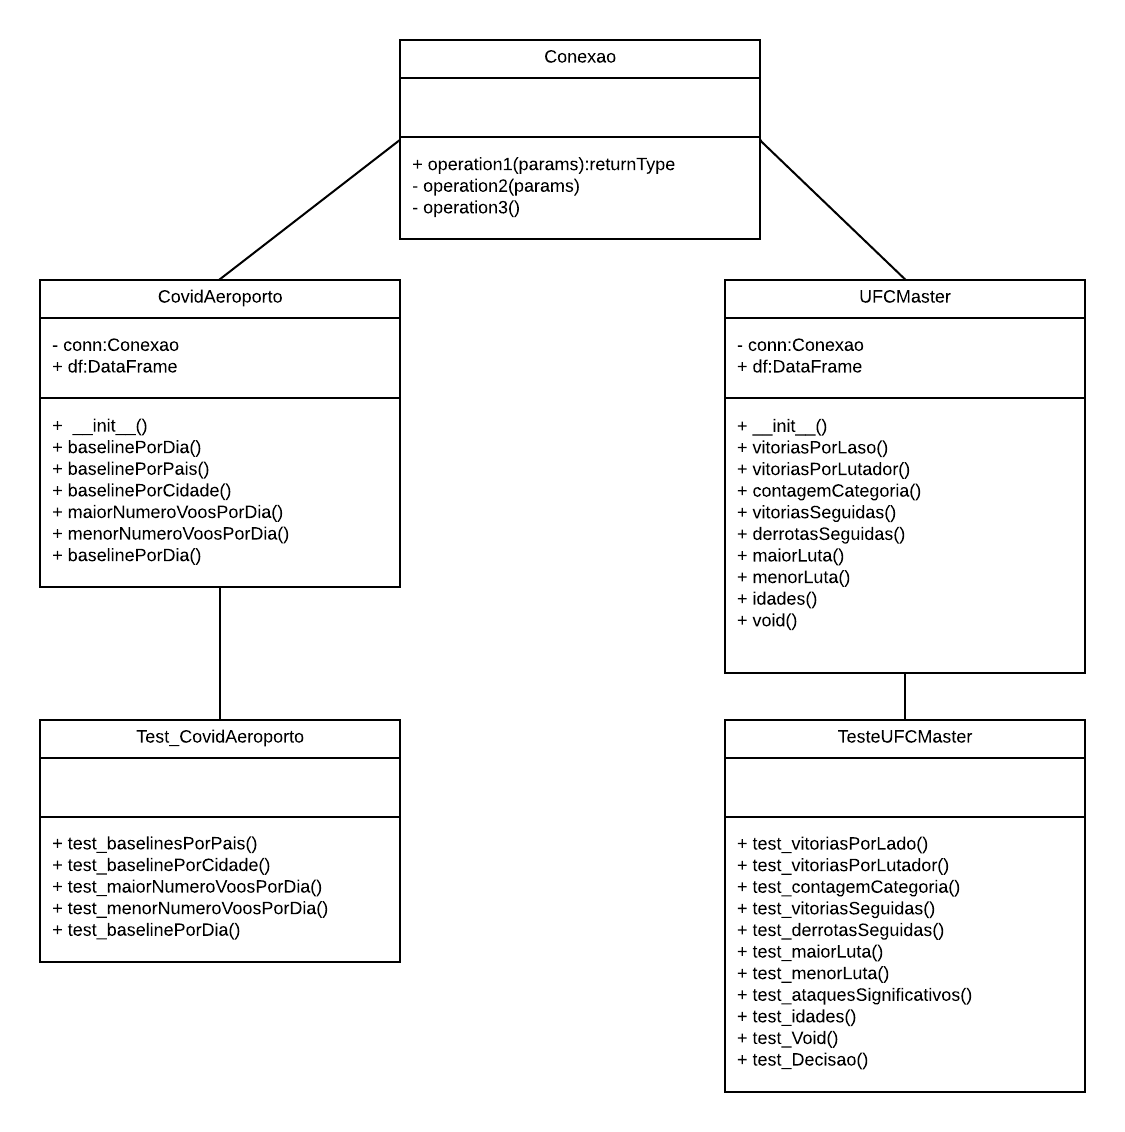
\includegraphics[scale = 0.8]{class-diagram.png} 
\end{figure}

\section{Análise dos dados}
\subsection{UFC}
A base de dados fornecida é composta de 4473 linhas e 136 colunas. A base fornece informações sobre o local, vencedor, idade dos lutadores, número de rounds da lutas, entre outros detalhes. Exploraremos os dados, de modo a compreender melhor o perfil dessas lutas. Inicialmente, analisaremos qual lado (vermelho ou azul) ganhou mais.

\begin{figure}[H] 
    \centering 
    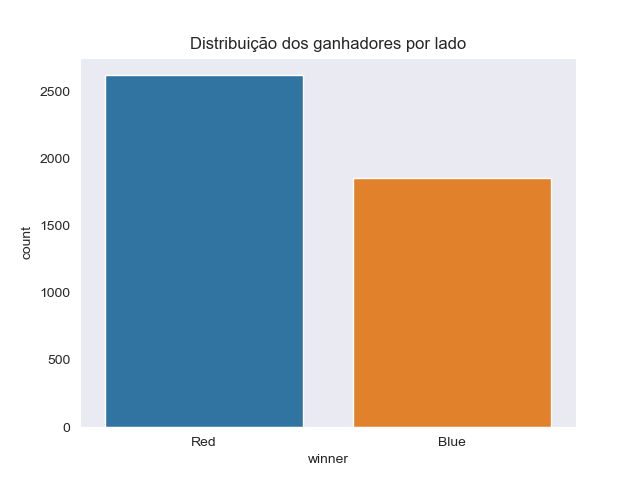
\includegraphics[scale = 0.7]{ganhador_lado.png} 
\end{figure}

\par Apesar de todas as lutas serem dueladas por um lutador vermelho e outro azul e os dois pertencerem a mesma categoria, pela visualização, o lado vermelho ganhou mais lutas com uma diferença considerável.
\par Outra informação importante é a distribuição dos lutadores por categoria, ou seja, para compreender o perfil das lutas, é necessário  ter conhecimento a cerca dos pesos dos jogadores. Analisaremos a disposição dos jogadores nas cinco categorias com maior número de integrantes.
    
\begin{figure}[H] 
    \centering 
    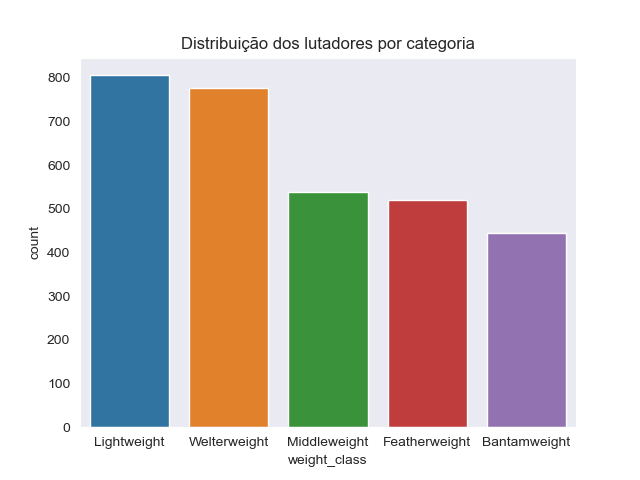
\includegraphics[scale = 0.7]{lutador_categoria.png} 
\end{figure}

\par As cinco categorias com maior número de integrantes são: Lightweight, Welterweight, Middleweight, Featherweight e Bantamweight. Dessa forma, a maior parte dos lutadores estão em categorias com peso limite baixos.
\par Após analisar as categorias com maior número de integrantes e o lado que venceu mais lutas, é interessante explorar quais lutadores ganharam mais lutas e quantas lutas ganharam. Do mesmo modo, é relevante analisar quais lutadores ganharam menos lutas e quantas lutas ganharam. Posteriormente, compararemos esses números e as diferenças entre esses lutadores.
    
\begin{figure}[H] 
    \centering 
    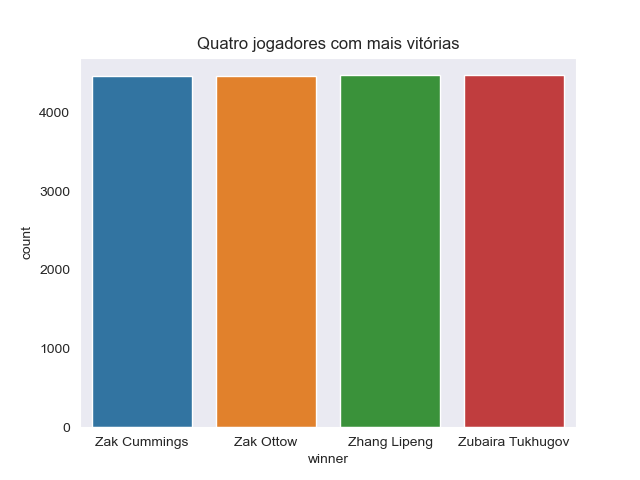
\includegraphics[scale = 0.7]{lutadores_mais_vitorias.png} 
\end{figure}
  
\par Os quatro lutadores com mais vitórias venceram mais de quatro mil lutas cada, sendo a diferença entre eles miníma. 

\begin{figure}[H] 
    \centering 
    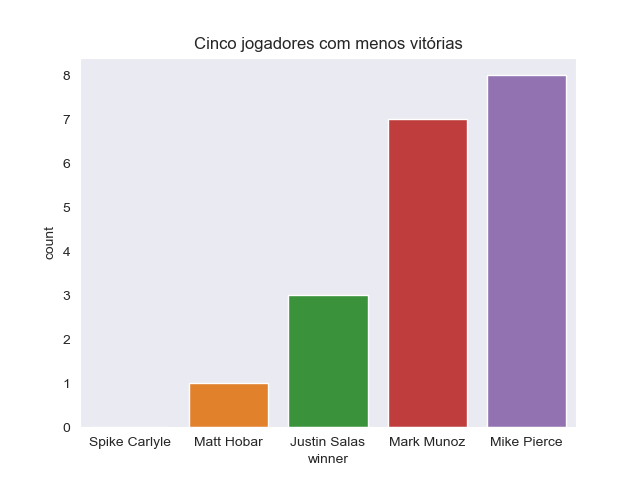
\includegraphics[scale = 0.7]{lutadores_menos_vitorias.png} 
\end{figure}

\par Já, os cinco lutares com menor número de vitórias ganharam menos de vinte lutas juntos. Desse modo, é discrepante a diferença entre os lutadores com maior rendimento e os lutadores com menos número de vitórias.
\par Após ter um conhecimento mais amplo sobre as características dos lutadores envolvidos, analisaremos se as lutas são longas ou curtas, ou seja, se possuem muitos rounds.

\begin{figure}[H] 
    \centering 
    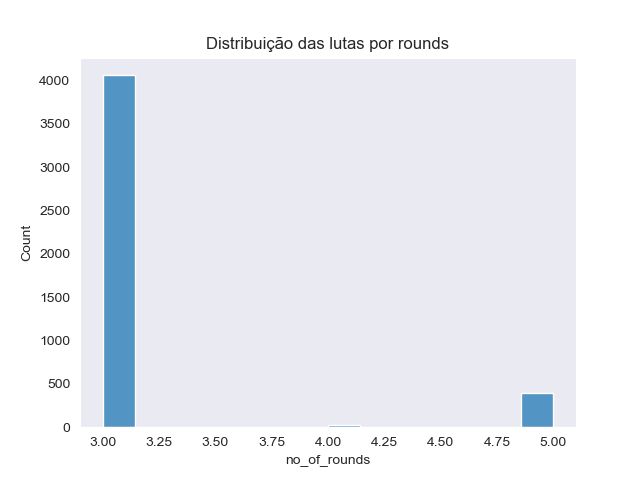
\includegraphics[scale = 0.7]{lutas_rounds.png} 
\end{figure}

\par A maior parte das lutas tiveram três rounds. 

\subsection{Impacto da COVID-19 no tráfego do aeroporto}
A base de dados fornecida é composta de 5936 linhas e 10 colunas. A base fornece informações sobre as transformações do fluxo de aviões devido a COVID-19. De modo análogo a base anterior, buscaremos compreender melhor esse dados. Inicialmente, analisaremos a data em relação a porcentagem da linha de base.

\begin{figure}[H] 
    \centering 
    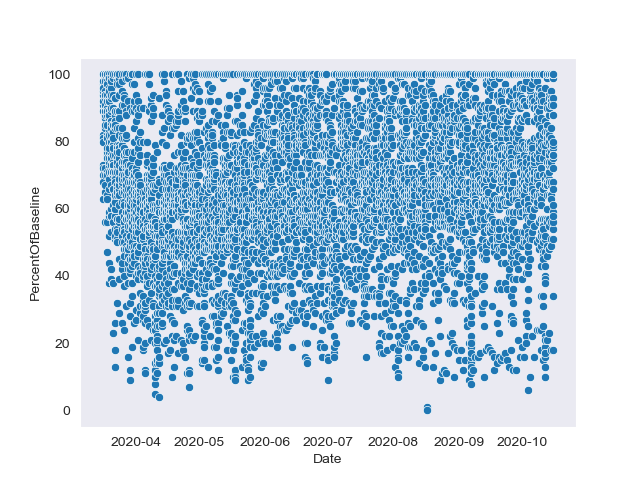
\includegraphics[scale = 0.7]{dias_percentofbaseline.png} 
\end{figure}

Por meio da visualização, é possível perceber nos meses de abril e maio houve um decréscimo da PercentOfBaseline. Esses meses correspondem ao início da pandemia. Assim, nesse período, a preocupação e medidas de isolamento estavam mais sólidas. Após março e abril, percebe-se que a PercentOfBaseline permaneceu sem bruscas alterações. 

\end{document}